\documentclass{article}

% if you need to pass options to natbib, use, e.g.:
%     \PassOptionsToPackage{numbers, compress}{natbib}
% before loading neurips_2020

% ready for submission
% \usepackage{neurips_2020}

% to compile a preprint version, e.g., for submission to arXiv, add add the
% [preprint] option:
%     \usepackage[preprint]{neurips_2020}

% to compile a camera-ready version, add the [final] option, e.g.:
%     \usepackage[final]{neurips_2020}

% to avoid loading the natbib package, add option nonatbib:
     \usepackage[nonatbib]{neurips_2020}
\raggedbottom
\usepackage[utf8]{inputenc} % allow utf-8 input
\usepackage[T1]{fontenc}    % use 8-bit T1 fonts
\usepackage{hyperref}       % hyperlinks
\usepackage{url}            % simple URL typesetting
\usepackage{booktabs}       % professional-quality tables
\usepackage{amsfonts}       % blackboard math symbols
\usepackage{nicefrac}       % compact symbols for 1/2, etc.
\usepackage{microtype}      % microtypography
\usepackage{graphicx}
\usepackage{caption, subcaption}
\usepackage{float,graphicx}


\title{
  A Recurrent Model of Approximate Enumeration \\
  \vspace{1em}
  \small{\normalfont Stanford CS238 Final Project}  % Select one and delete the other
}
% The \author macro works with any number of authors. There are two commands
% used to separate the names and addresses of multiple authors: \And and \AND.
%
% Using \And between authors leaves it to LaTeX to determine where to break the
% lines. Using \AND forces a line break at that point. So, if LaTeX puts 3 of 4
% authors names on the first line, and the last on the second line, try using
% \AND instead of \And before the third author name.

\author{
  Gabe Barney \\
  Symbolic Systems \\
  Stanford University \\
  \texttt{barneyga@stanford.edu} \\
  \and
  \bf{Griffin Young} \\
  Symbolic Systems \\
  Stanford University \\
  \texttt{gcyoung@stanford.edu} \\
}

\begin{document}

\maketitle

\begin{abstract}
Many animals have the ability to subitize--that is, to rapidly and exactly assess the number of items in a small set (typically less than 5). This has traditionally been considered a separate ability from the Approximate Number System, which allows for approximate estimation of the number of items in a set. Recently, a  unified theoretical model was proposed which accounts for the qualitative change in accuracy and speed above the subitizing threshold through a Bayesian model of information gathering under resource constraints \cite{unified}. In this paper, we  provide a concrete implementation of this theoretical model by using a modified version of the Recurrent Attention Model (RAM), a recurrent neural network which can direct its attention to different points in an image across several steps of processing. We find that, as predicted by the Bayesian model, underestimation occurs in an imbalanced dataset in lower-capacity models and at earlier timesteps. 
\end{abstract}

\section{Introduction}
Numerical cognition is a field of neuroscience that is being transformed by the use of connectionist models for modeling the brain. One foundational question in this field is the basis of the Approximate Number System. This is the ability of humans and animals to estimate the number of objects in the field of view. In 2012, researchers found neurons in a Deep Neural Network trained only to reconstruct an input image whose responses had a monotonic relationship with numerosity \cite{zorzi}, mirroring the response profiles of neurons in the Lateral Intraparietal Area of macaques \cite{roitman}.

More recently, Convolutional Neural Networks pretrained on ImageNet but naive to explicit numerosity training have been shown to have peaked responses to particular numerosities and a graded decrease in response to adjacent numerosities \cite{dewind}\cite{nasr}. These findings mirrored the tuning properties of neurons in the Ventral Intraparietal Area of nonhuman primates \cite{merten} and humans \cite{kutter}.

The temporal characteristics of numerosity processing have not received as much modeling attention. Previous models, with one exception, have assumed a single parallel extraction of numerosity from an image. The one notable exception being \cite{mcclelland}, though no analysis of the temporal dynamics of the network were presented and the DRAW model allows the model to dynamically alter the shape of the glimpse it takes, unlike biological vision. This is a notable gap in the literature considering the evidence that human numerosity estimates become more accurate over time \cite{gilmore} and with the number of dots foveated \cite{accumulator}.

In this work, we model human approximate number perception with a recurrent neural network which chooses, at each time step, a location in the image at which to center its fovea.

\subsection{A Unified Account of Numerosity Perception}
The theoretical framework we will use to interpret the behavior of the network comes from a paper by Cheyette and Piantadosi (2020) \cite{unified}. In it, they accounted for several key psychophysical features of the approximate number system with a Bayesian framework, in which a prior over possible numerosities is updated over time at a certain information gathering rate up to a certain information bound. Specifically, the distribution over the predicted numerosity k given the actual numerosity n, Q(k|n), is chosen to minimize the expected divergence from the veridical numerosity, bounded by divergence from a prior over the probability of encountering a given numerosity P(n). This allows the Approximate Number System and subitizing to be explained by a single mechanism: subitizing just occurs for numbers who fall within the information bound of the prior.
\subsection{Goals}
We will operationalize the information bound as the size of the hidden layer of the RNN. We will train several models with different hidden layer sizes and test the following hypotheses, pulled from \cite{unified}:
\subsubsection{Hypothesis 1: Scalar Variability: Larger sets exhibit larger variability in numerosity estimates.}
This is a standard psychophysical finding in humans and animals. Larger set sizes will have more variable numerosity estimates.
\subsubsection{Hypothesis 2: Subitizing: Rapid and exact enumeration of small sets.}
Small numerosities will be enumerated with very low error and relatively quickly due to the low KL divergence between the power law distribution of numerical frequency (that is, lower numbers are seen more frequently than higher numbers) and the posterior distribution for images with low set sizes.
\subsubsection{Hypothesis 3: Subitizing range varies with information bound.}
The size of the information bound, operationalized as the size of the hidden layer in the RNN, will determine the cutoff point for the subitizing range. That is, models with larger hidden layers will have a larger range with extremely low error, followed by a transition point to a range of numbers exhibiting scalar variability.
\subsubsection{Hypothesis 4: Underestimation of numerosity at lower information bounds.}
Again due to the power law distribution, we expect underestimation at lower information bounds.
\subsubsection{Hypothesis 5: Worse, and underestimated, predictions at earlier time steps.}
This is for the same reason as for the lower information bounds, since the constraint is the minimum of the information bound and the value Rt, where R is a linear information extraction rate and t is the number of time steps.

\section{Related Work}
\subsection{DRAW: A Recurrent Neural Network For Image Generation}
The model that has inspired the use of foveated input is the \textit{Deep Recurrent Attentive Writer} (DRAW)\cite{draw} architecture. The DRAW model was used by DeepMind to incorporate a mechanism that emulates the foveation of the human eye with a sequential variational autoencoder framework to generate complex images iteratively. The temporal nature of RNNs causes this architecture to provide it with the iterative image construction being more life-like than other approaches to image generation.

\begin{figure}[ht]
\begin{center}
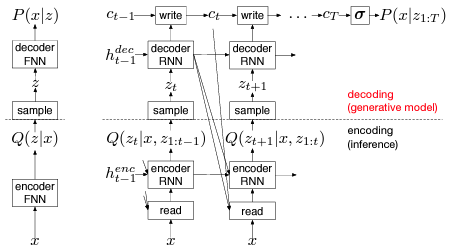
\includegraphics[]{VAE--DRAW.png}
\caption{\textbf{Left:} Conventional VAE ~~~~~~~~~~ \textbf{Right:} DRAW}
\end{center}
\end{figure}

The architecture of DRAW is a slight alteration to the conventional variational autoencoder. Instead of the encoder and decoder being feedforword neural networks, they are LSTM RNNs. These RNNs take input from the previous encoders and decoders by means of a canvas matrix, which can be partially updated rather than completely generated due to selective attention.

Generating images iteratively enables selective attention to parts of the image. The main challenge is directing that selective attention. DRAW applies an array of 2D Gaussian filters to the image, which varies the location, zoom, and resolution of the attention based on the output of the decoder LSTM.
% \begin{figure}
% \begin{center}
% 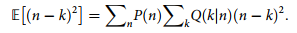
\includegraphics[]{eq1.png}
% \caption{Equation 1: The expected distance between the perceived and actual numerosity.}
% 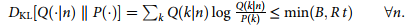
\includegraphics[]{eq2.png}
% \caption{Equation 2: The KL Divergence between the prior over the probability of each numerosity and the posterior distribution must be below the minimum of an information bound B and the product of an information gathering rate R and the number of time steps t.}
% 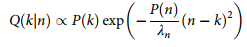
\includegraphics[]{eq3.png}
% \caption{Equation 2: The result of minimizing equation 1 bounded by equation 2.}
% \end{center}
% \end{figure}
% Thus, the approximate number system is modeled as the result of minimizing equation 1 subject to the bound of equation 2, yielding equation 3.\newline


\subsection{Can Generic Neural Networks Estimate Numerosity Like Humans?}
Chen, et al. (2018) \cite{mcclelland} investigated how well the characteristics of experimental data about the approximate number system would emerge in a standard feedforward network and in a modified version of the DRAW  model. The experimental data had shown that there is a constant coefficient of variation for numerosities larger than four, even in datasets without imbalanced numerosities. They found that the sequential nature of the model was not used, as "the focus of attention remained constant over
glimpses, and the accuracy of estimates was almost as good
on the first as on the last glimpse."\newline
In this paper, we wanted to focus moreso on the temporal aspect of glimpses, and determining how time affects the models understanding. , so we chose the RAM model instead of the DRAM model. We discuss DRAM in section 3.5.



\subsection{Numerosity discrimination in deep neural networks: Initial
competence, developmental refinement and experience
statistics}
Humans, non-humans, and their babies can all detect changes in numerosity. This is evidence for the innate number system. The possibility for neural network modeling sheds light on potential explanations for why numerical acuity improves with cognitive development. In this paper, Testolin, et al. (2019) \cite{competence} substantiates the basis of the innate number system by showing that neural networks exhibit numerosity sensitivity without training and that numerical acuity is improved our time through training. Their main finding was that animals may not necessarily have dedicated systems for numerosity, because their use of a general neural network demonstrates that a general system can provide this processing, rather than an evolutionarily-based approximate number system.


\subsection{Recurrent Models of Visual Attention (RAM): }
Mnih, et al. (2014) \cite{deepmind} presents the Recurrent Attention Model. Its objective is to recognize objects in images with a deep recurrent neural network via reinforcement learning. At each time step, it received several patches of an input image at different resolutions, centered around some point in the image. It updates its hidden layer and then outputs an output distribution over the target classes as well as a distribution over the next center from which the next patches are sampled.


\subsection{Multiple Object Recognition with Visual Attention (DRAM): }
Ba, et al. (2015) \cite{DRAM} presents the Deep Recurrent Attention Model. Clearly an alteration of the RAM model by merely inspecting the name. Its objective is to recognize multiple objects in images with a deep recurrent neural network via reinforcement learning, similarly to the RAM model. Its results showed that it was better than the state-of-the-art convolutional neural networks at the time, and used less resources and computation.

RAM is more in line with the domain we chose to look into, as it determines gazing strategies of the images, but finds particular challenges with real world challenges. These numerosity estimation tasks do fall into tasks that RAM is able to model, and so we figured that focusing on gazing and temporal aspects was more important, as well as it is more simplisitic and similar to human behavior.

\subsection{Enriched Deep Recurrent Visual Attention Model for Multiple Object
Recognition (EDRAM): }

A recent paper that we have looked into is the paper that introduces the Enriched Deep Recurrent Visual Attention Model. Ablavatski, et al. (2017) \cite{EDRAM} developed an improvement to DRAM and is fully differentiable. The important aspect about this, is the use of the the Spatial Transformer and improved upon the state-of-the-art. Transformers have made a big impact on Natural Language Processing and Computer Vision, so this paper introduces the possibility of applying transformers to this domain.




\section{Methods}

\subsection{Datasets}
\begin{figure}[ht]
\begin{center}
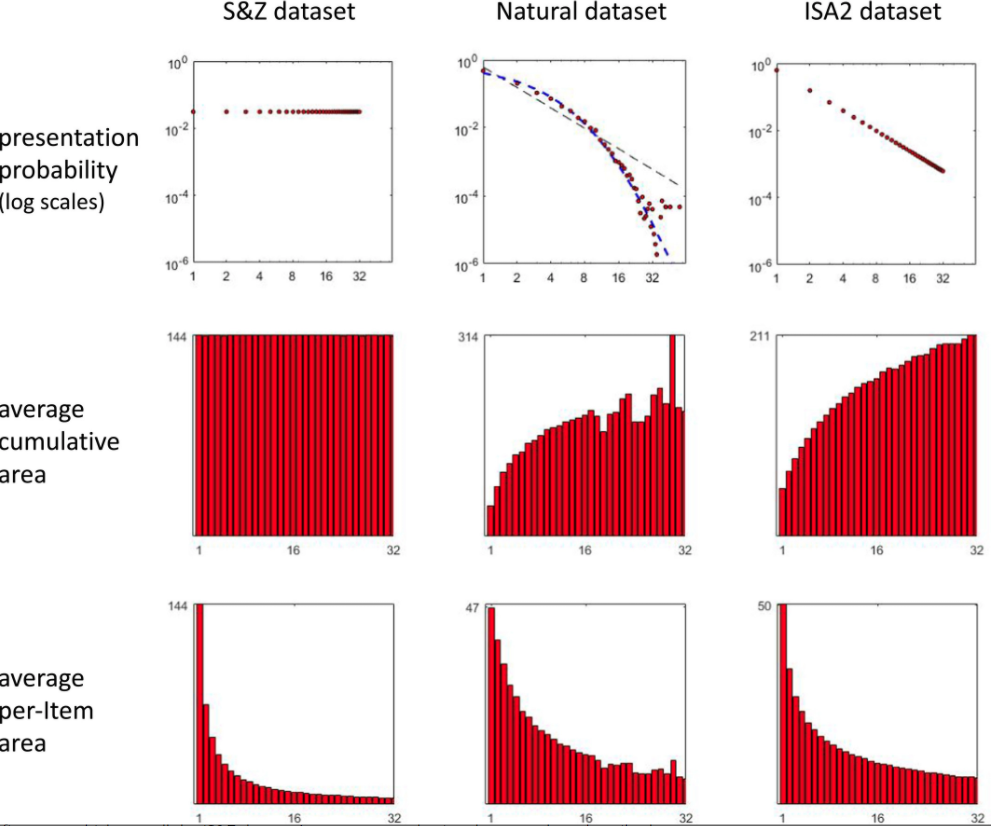
\includegraphics[scale=.38,width=0.3\linewidth]{dataset.png}
\caption{}
\label{dataset}
\end{center}
\end{figure}
Jay McClelland generously provided the three datasets in figure \ref{dataset}, though we only trained on the Natural and S+Z datasets. The figure summarizes the differences, and full details are available in \cite{competence}. Essentially, each contains binary images of varying numbers of white rectangles on a black background. The Natural dataset has a power law distribution, where the frequency of a number n is about $\frac{1}{n^2}$ the frequency of the number 1. The dataset was split into 771840 training samples, 85760 validation samples, and 214400 test samples. The S+Z dataset has a uniform distribution across numbers. We split it into 36864 training samples, 4096 validation samples, and 10240 test samples.

\subsection{Model}

The model we chose is the Recurrent Attention Model (RAM) from \cite{deepmind}. The core is a recurrent neural network which, at each time step, takes in a foveated 'glimpse' of an input image and outputs: 1) a Gaussian distribution over fovea centers from which the fovea center at the next time step is sampled, 2) a softmax distribution over some classes, and (our novel contribution), 3) a Bernoulli distribution from which a STOP action is sampled, either 1 to continue computation or 0 to halt. The model is trained with the REINFORCE update rule, which adjusts the parameters of the network so that actions which have led to high reward become more probable.\newline
We used an open source RAM implementation \cite{kevinzakka} as our jumping off point. Instead of giving a reward of 1 to every glimpse step if the final glimpse classified the image correctly, we give a reward of 1 only to the first time step whose STOP action was a 0, and we give a penalty to each time step whose STOP action was a 1. \newline
Our final analysis uses only the original RAM implementation without the STOP action. We found that including any penalty per timestep caused the network to immediately stop computation, not allowing us to examine the evolution of the prediction across time steps. We did include one alteration to the RAM model: instead of only calculating the reward based on the prediction at the final timestep, we calculated the reward based on the predictions at every time step. This incentivized the model to output as accurate an answer as it could at every time step.\newline
\subsection{Training}
We trained three models, with hidden layers of 64, 256, and 2560, in Google Colaboratory. Patches of the image, centered around the model-chosen fovea center at each time step, were of size 3x3, 12x12, and 48x48, the latter two average-pooled to be 3x3 as well. Each image was viewed for 15 timesteps. We trained the models for 10, 20, and 10 epochs respectively with an ADAM optimizer with initial learning rate 0.0003. Testing was done on the versions of each model with the highest validation accuracies.


\section{Results}
\begin{figure}[H]
  \begin{subfigure}{0.6\textwidth}
  \centering
    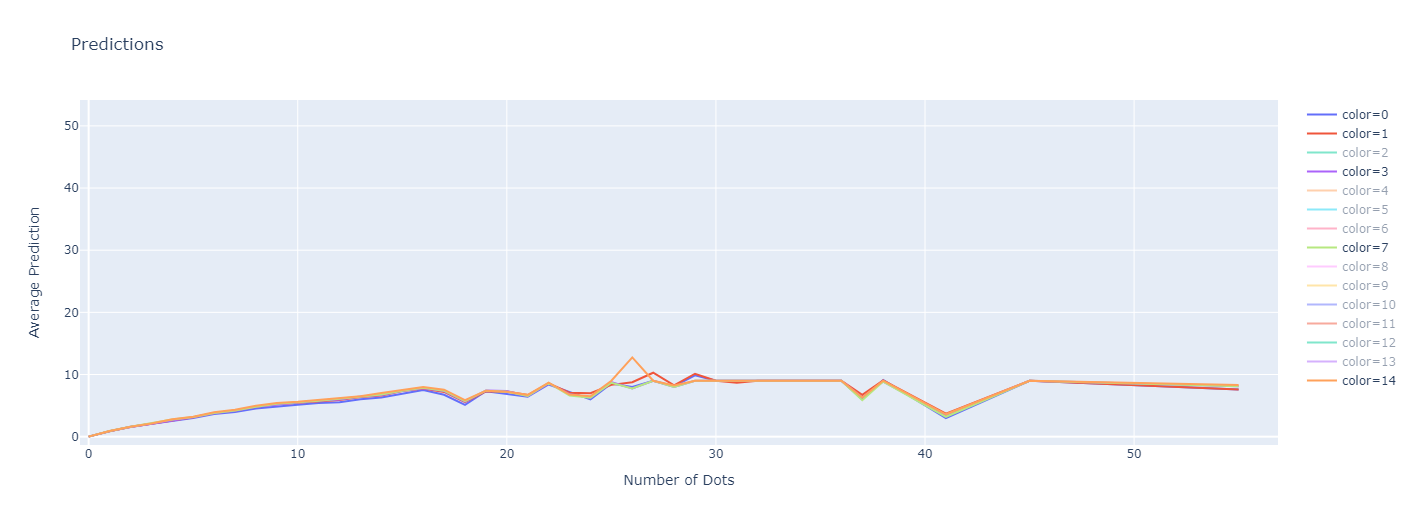
\includegraphics[width=.8\linewidth]{template/fourthx_0to55_prediction_samescale.png}
    \caption{Hidden size 128 Predictions}
    \label{fig:1}
  \end{subfigure}%
  \begin{subfigure}{0.6\textwidth}
    \centering
    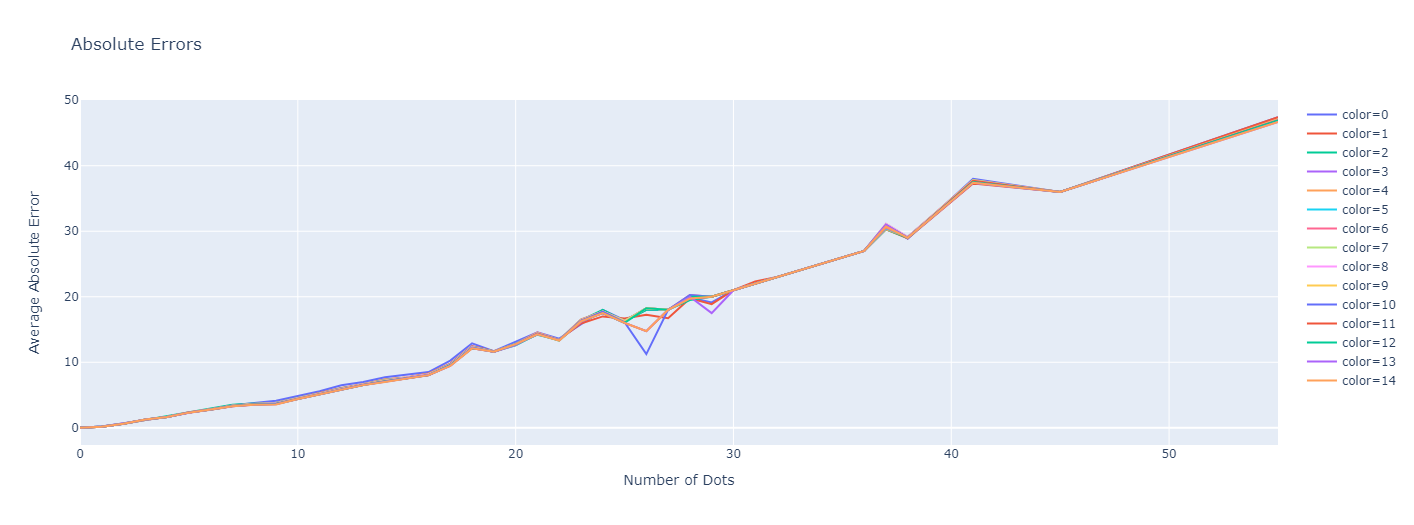
\includegraphics[width=.8\linewidth]{template/fourthx_0to55_error_samescale.png}
    \caption{Hidden size 128 Errors}
    \label{fig:4}
  \end{subfigure}
  
  \medskip
  \begin{subfigure}{0.6\textwidth}
    \centering
    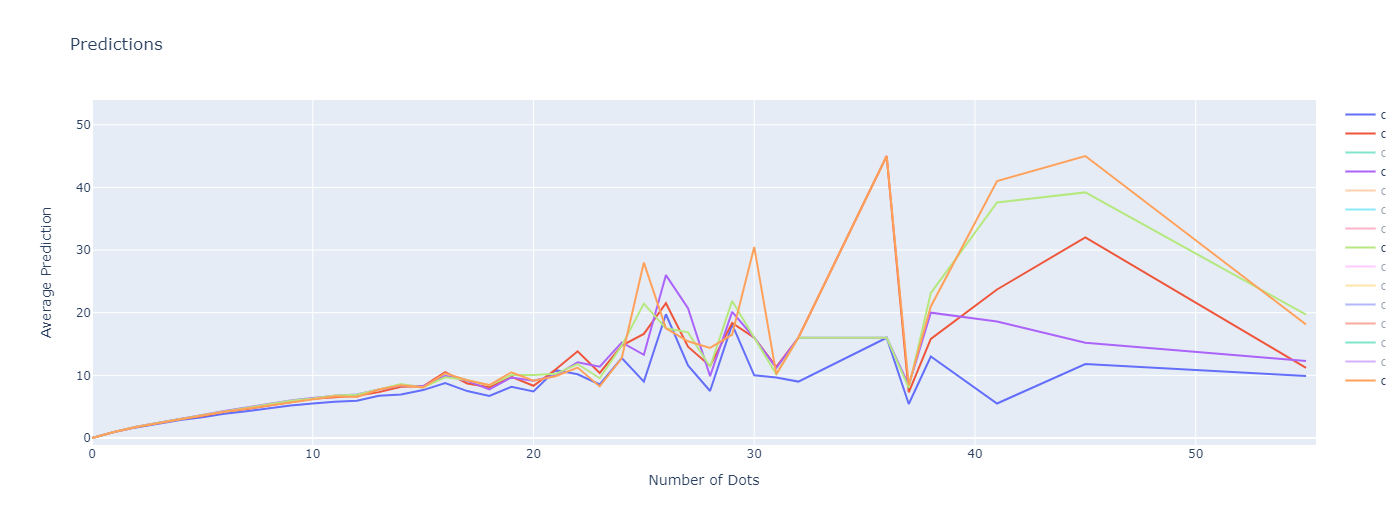
\includegraphics[width=.8\linewidth]{template/1x_0to55_prediction_samescale.png}
    \caption{Hidden size 256 Predictions}
    \label{fig:2}
  \end{subfigure}
    \begin{subfigure}{0.6\textwidth}
    \centering
    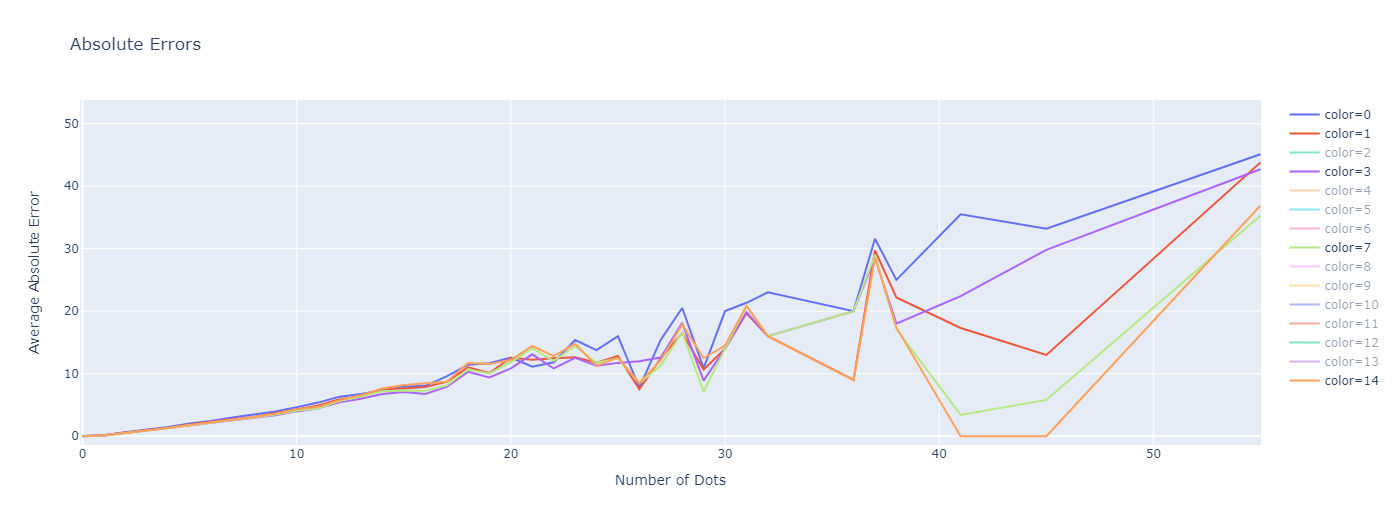
\includegraphics[width=.8\linewidth]{template/1x_0to55_error_samescale.png}
    \caption{Hidden size 256 Errors}
    \label{fig:5}
  \end{subfigure}
  
  \medskip

  \begin{subfigure}{0.6\textwidth}
    \centering
    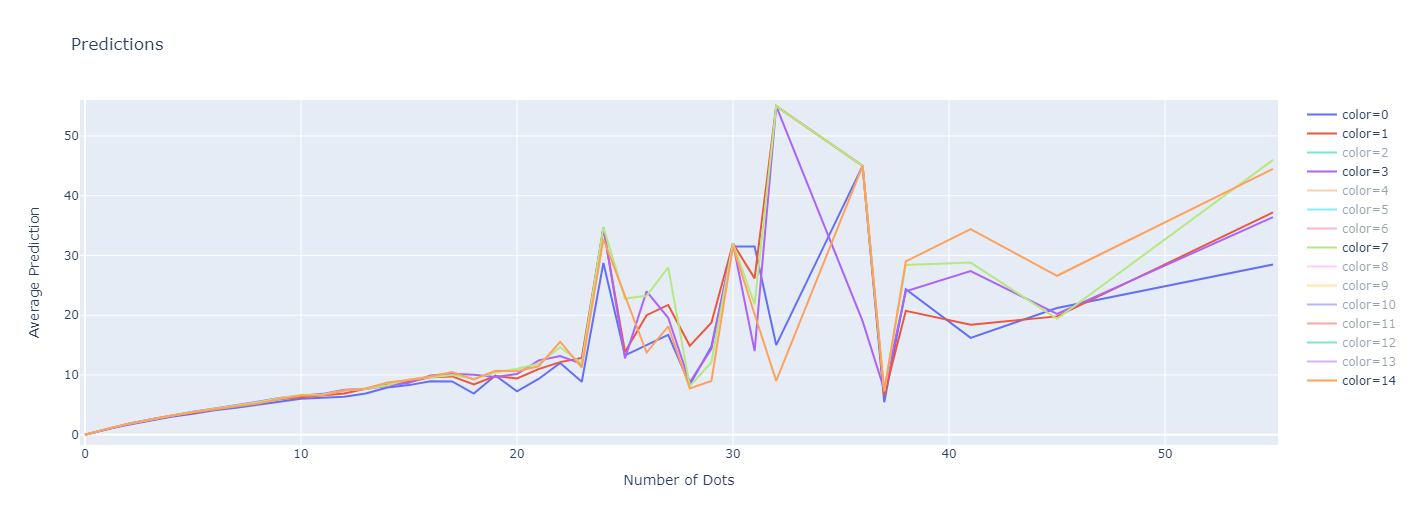
\includegraphics[width=.8\linewidth]{template/10x_0to55_prediction_samescale.png}
    \caption{Hidden size 2560 Predictions}
    \label{fig:6}
  \end{subfigure}
  \begin{subfigure}{0.6\textwidth}\quad
    \centering
    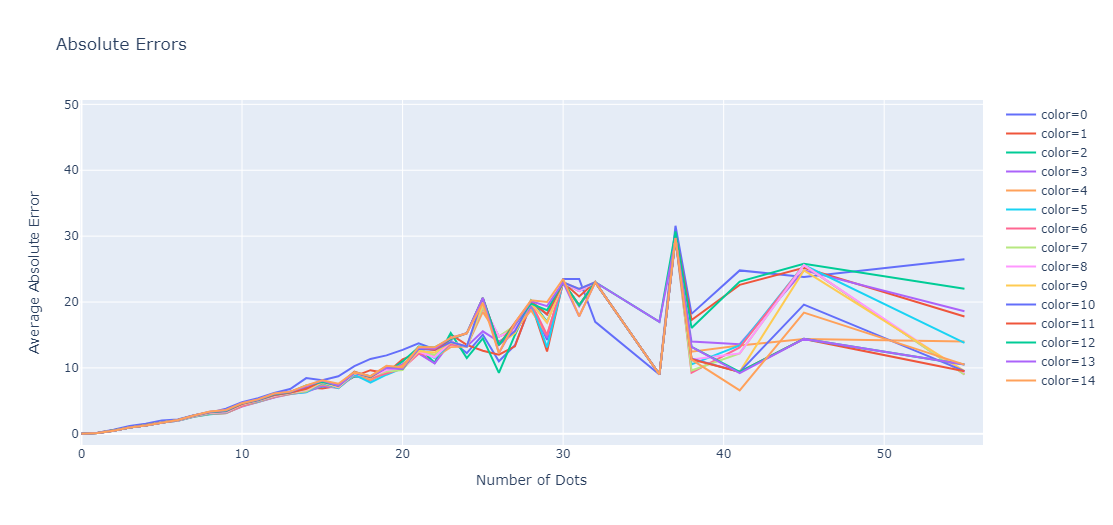
\includegraphics[width=.8\linewidth]{template/10x_0to55_error_samescale.png}
    \caption{Hidden size 2560 Errors}
    \label{fig:3}
  \end{subfigure}
  \caption{Natural dataset, with power law frequencies across numbers. Predictions and errors averaged across images with the same number of dots at each time step. Each different colored line is a different timestep.}
  \label{fig:images}
\end{figure}

\newpage

\subsection{Hypotheses}
\begin{itemize}

    \item \textbf{Hypothesis 1: Scalar variability}\newline
    We found evidence for this hypothesis. For all models but the first, the standard deviation of the predictions increases with the numerosity. 
        \begin{figure}[H]
  \begin{subfigure}{0.3\textwidth}
    \centering
    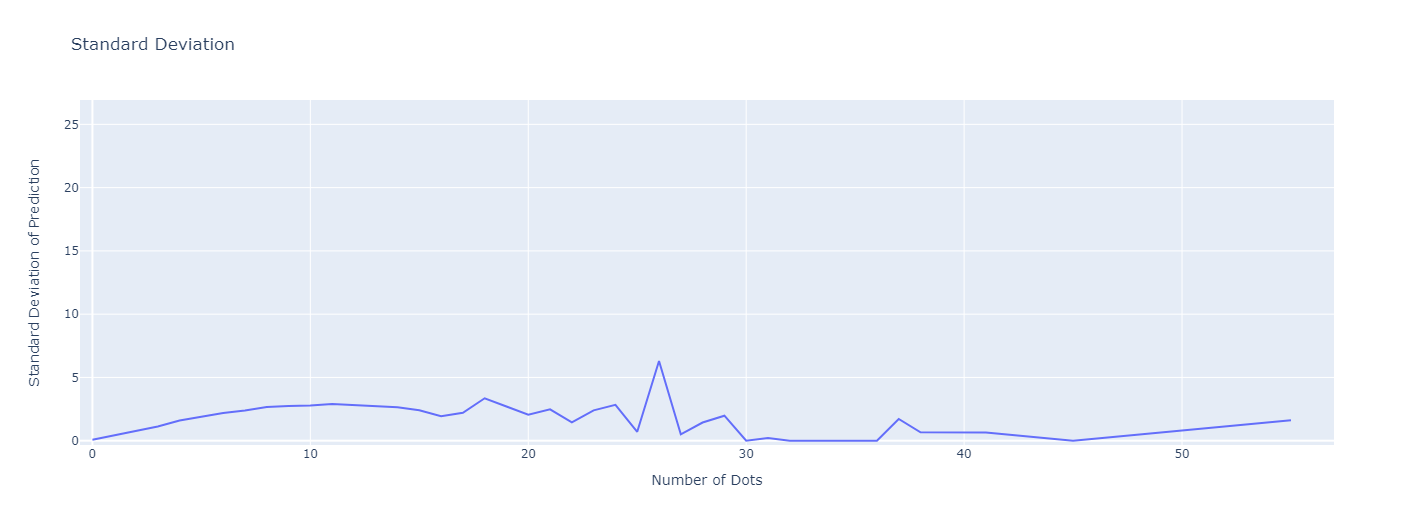
\includegraphics[width=.8\linewidth]{template/fourthx_std.png}
    \caption{Hidden size 128}
    \label{fig:6a}
  \end{subfigure}
  \begin{subfigure}{0.3\textwidth}\quad
    \centering
    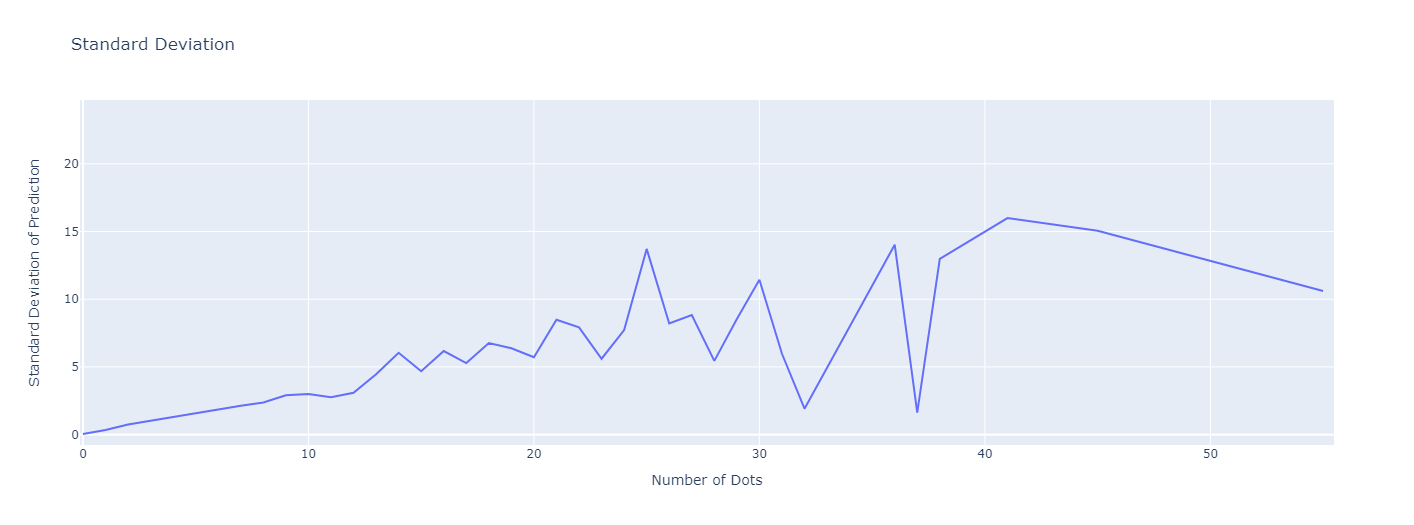
\includegraphics[width=.8\linewidth]{template/1x_std.png}
    \caption{Hidden size 256}
    \label{fig:3a}
  \end{subfigure}
  \begin{subfigure}{0.3\textwidth}\quad
    \centering
    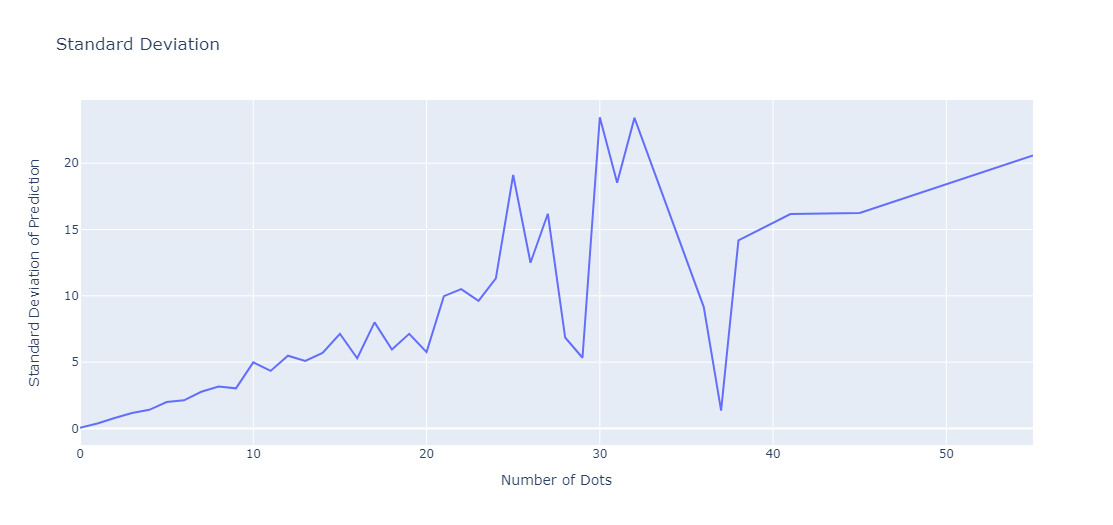
\includegraphics[width=.8\linewidth]{template/10x_std.png}
    \caption{Hidden size 2560}
    \label{fig:3b}
  \end{subfigure}
  \caption{S+Z dataset, with equal freqeuncies across numbers. Standard deviations of predictions averaged across timesteps for each numerosity.}
  \label{fig:images-a}
\end{figure}
    \item \textbf{Hypothesis 2: Subitizing}\newline
    We did not find evidence for this phenomenon in our models.\newline
    Without the stop action, we cannot make claims as to the rapidness while within the subitizing range, but we can say that there is stronger confidence of the model in its predictions at lower numerosities. That is, there is less divergence between the predictions between timesteps at lower numbers of dots presented in the images. \newline
    In terms of accuracy, we reproduced previous findings failing to replicate the human-like near-perfect classification accuracy for numbers 2-4 in neural models \cite{mcclelland}.
    
    \item \textbf{Hypothesis 3: Subitizing range increases with information bound}\newline
    We did not find support for this hypothesis, since the subitzing range for all the models was the same: only the number 1. \newline
    With a more generous classification of subitizing as anything with less than 1 absolute error, there is a small, yet present, difference in the subitizing ranges between information bounds. Our largest hidden layer sizing has an absolute error of less than 1 at its best timestep until 4 dots are presented, while our smallest size has an absolute error of less than 1 at its best timestep until 3 dots. This is just reflective of a larger trend of lower error in the models with larger hidden layers.
    
    \begin{figure}[H]
  \begin{subfigure}{0.6\textwidth}
    \centering
    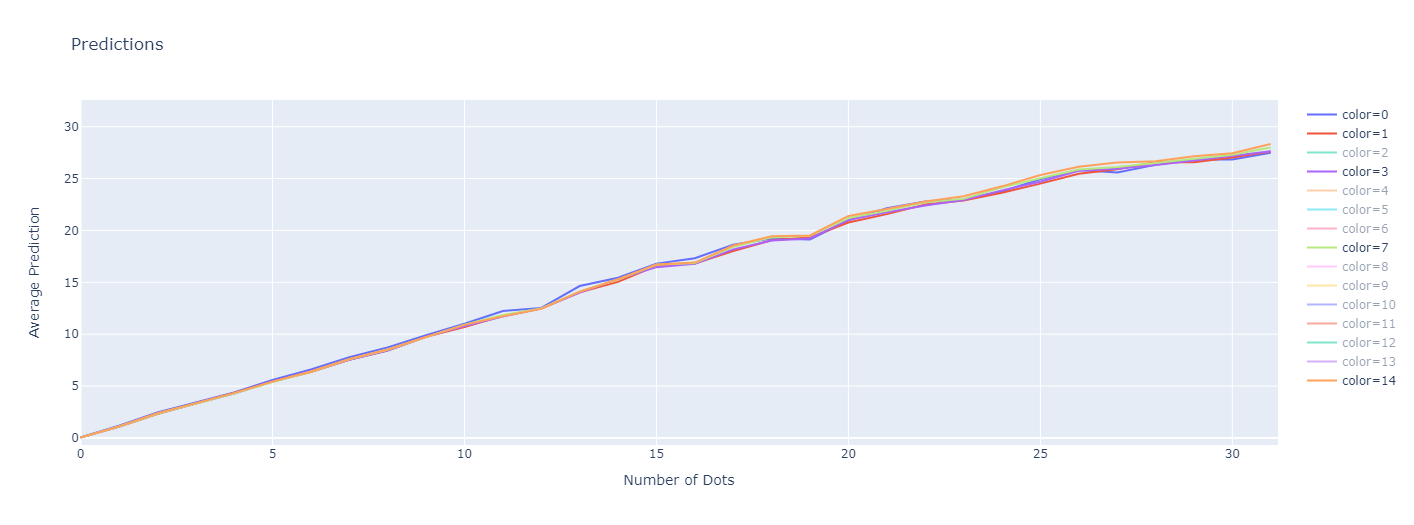
\includegraphics[width=.8\linewidth]{template/sz_10x_prediction.png}
    \caption{Hidden size 2560 Predictions}
    \label{fig:6b}
  \end{subfigure}
  \begin{subfigure}{0.6\textwidth}\quad
    \centering
    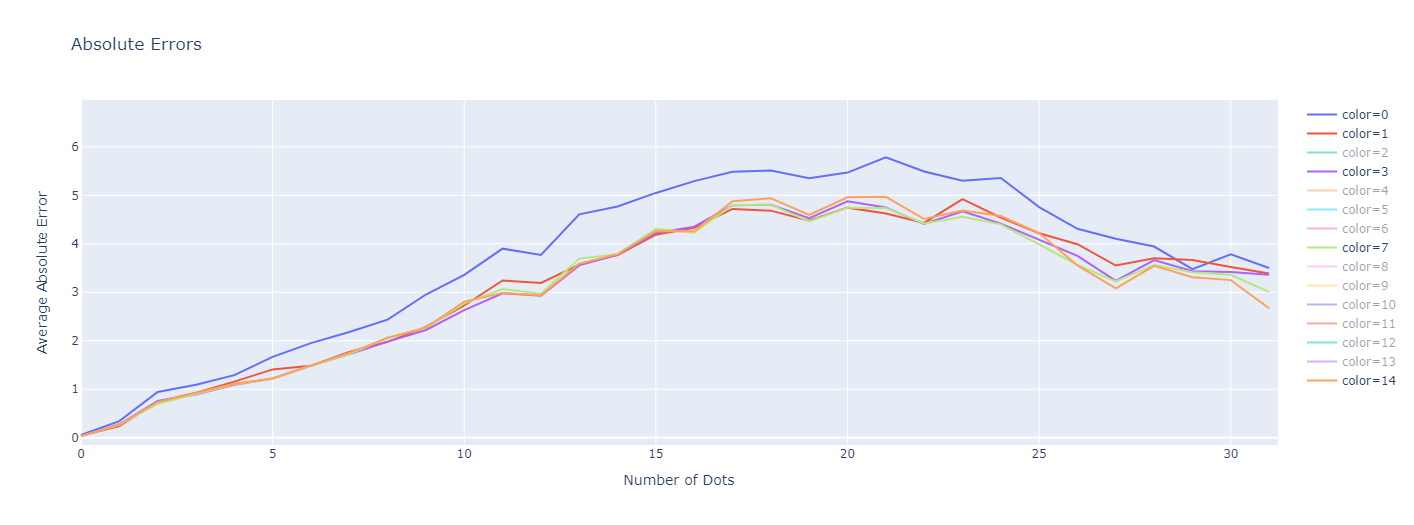
\includegraphics[width=.8\linewidth]{template/sz_10x_error.png}
    \caption{Hidden size 2560 Errors}
    \label{fig:3c}
  \end{subfigure}
  \caption{S+Z dataset, with equal freqeuncies across numbers. Predictions and errors averaged across images with the same number of dots at each time step. Each different colored line is a different timestep.}
  \label{sz}
\end{figure}

    \item \textbf{Hypothesis 4: Underestimation at lower information bounds}\newline
    We did find evidence to support this hypothesis. There is a progressive decrease in underestimation as the hidden layers size, or information bound, is increased. This is especially notable in contrast to the S+Z dataset in Figure \ref{sz}, in which the average estimate is actually an overestimation.
    
    \item \textbf{Hypothesis 5: Underestimation at earlier timesteps}\newline
    We did find evidence to support this hypothesis.
    We find in the majority of cases on our largest hidden layer model and in every case on our average model that timestep 0 produces the worst performing predictions. Especially in the larger numerosities, we also find a graded increase in predictions as the timesteps progress, with the final timestep having the highest prediction. \newline
    This is especially interesting in contrast to the balanced S+Z dataset in Figure \ref{sz}, in which, at the smaller numerosities, timestep 0 is an overestimate compared to the final timestep, but at larger numerosities, timestep 0 is an underestimate. This supports the hypothesis that the model maintains a prior over the probability of each numerosity appearing which it updates over time to be more consistent with the evidence it accumulates. This prior has more mass in the lower numerosities for the Natural dataset, causing underestimation for higher numbers. In the balanced S+Z dataset, however, the prior has equal mass over all numerosities, causing lower numerosities to be overestimated and higher ones to be underestimated.
\end{itemize}


\section{Discussion}
\begin{figure}[H]
    \centering
    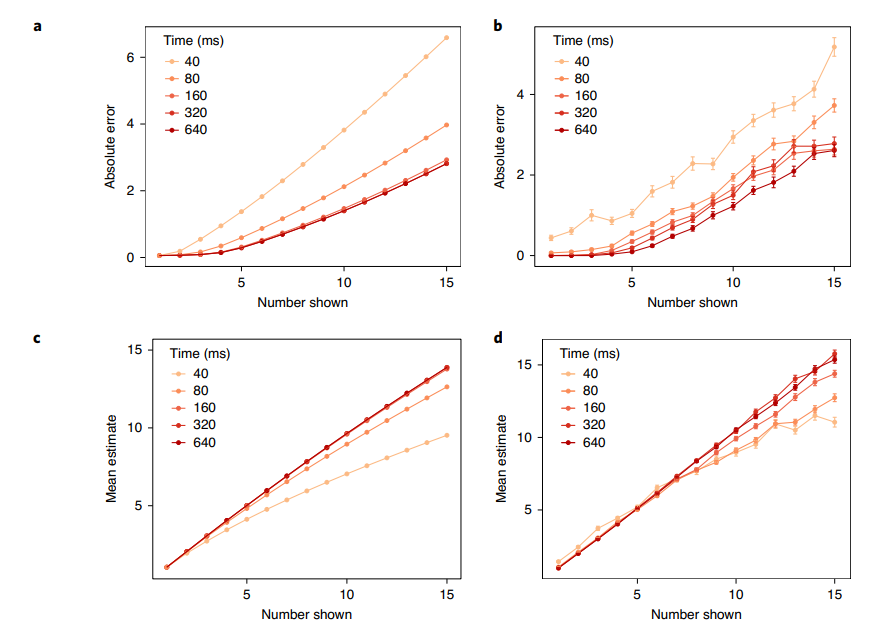
\includegraphics[width=0.8\linewidth]{template/unified.png}
    \caption{Graph from \cite{unified}. The left shows the theoretical model's predictions (top) and error (bottom) for different exposure times. The right shows the same but for human data.}
    \label{fig:unified_graph}
\end{figure}
Aside from the subitizing range, our results look very similar to those in Figure \ref{fig:unified_graph} for both the theoretical model and the human results. When trained on the imbalanced Natural dataset, our models consistently underestimated the numerosity of the images, especially at earlier timesteps. When trained on a balanced dataset, this pattern shifted to be one of overestimation at lower numbers and underestimation at higher numbers. This is consistent with the unified model presented in \cite{unified}, in which a prior over numerosities reflecting the frequency of exposure in the dataset is updated over time. \newline
Additionally, by training three models with different hidden layer sizes, we found limited support for the hypothesis that the different subitizing ranges between infants, adults, and chimpanzees are the result of different visual memory capacities. Though none of our models had a subitizing range larger than 1, we did find that the error for both of the larger models was smaller across numerosities. It's possible that an even higher capacity model would push this error down even farther, causing more than just the first number to have near-zero estimation error and thus extending the subitizing range. \newline
Curiously, despite the increase in accuracy across time steps (especially between the first and the second), we found that, as in previous work, the model did not effectively manipulate the location of its retina \cite{mcclelland}, preferring instead to leave it in mostly the same place in the upper left hand corner of the image. This makes the behavior of the model difficult to compare to humans, who do strategically move their gaze around an image. We were unable to determine why this capability was not used. \newline
Finally, a word about the project of modeling human behavior with deep neural networks:\newline
An issue that we find with our lower hidden layer sizing models is the lack of a notable divergence between timesteps for their predictions. We believe this is because different information bounds reach their capacity for learning this problem at different rates, and the number of epochs they were ran for were either too few or too many. If it were too few, the model may have been able to sufficiently learn from additional timesteps, producing nearly the same results. Or, if it were overtrained, then it may have been able to learn its best numerosity predictions at each timestep, so new timestops do not yield any improvement in performance. This yields some additional discussion.

We question the value of if we should train the RAM model, and if so, how many epochs? These are issues of what is the most effective way to think about RAM's simplistic emulation of human glimpses for this task? It makes sense that numerosity estimation would improve with age \cite{mcclelland}, and we could think of a fresh RAM model as a newborn child. We do witness some of the hypotheses in models that were trained for a single epoch, but with more epochs the model becomes far more effective in making guesses outside of its subitizing range. But if the models are trained too much, the absolute error throughout this task stays the same no matter the number of dots presented, which does not support the two-system model. It's a very intricate balance, as there is no right or wrong answer for what is the right choice, although it does seem like if we want a reasonable conjugate to human abilities we would have to train the model, but we cannot allow it to become too good at its task, as so it outdoes humans.



\section{Conclusions And Future Work}
In our concrete model of sequential number estimation, we found evidence to support two key claims made in \cite{unified}: that underestimation occurs in systems with lower information bounds and at shorter exposure times due to the imbalance in exposure to different numbers in natural images. Since the subitizing range was the same for all of our models (including an unpublished run with 10,240 neurons in the hidden layer), we were unable to make any conclusions about the effect of visual memory capacity on subitizing range except to say that our higher capacity models did have lower errors across all numerosities, including 2-4, and it's possible that an even higher capacity model would be able to improve performance to the point of extending the subitizing range. This is a promising avenue of further research and would provide compelling evidence for a one-system account of subitizing and approximation.\newline
This Recurrent Attention Model is notably simplistic, and so there are questions as to what changes are necessary to make it a better model of human behavior. There has been many large leaps in modeling since RAM was introduced in 2014, so we may have missed a more effective method, or there is new modeling techniques that could be leveraged into being applied in this domain. Exploring other modeling options could be fruitful, yet we want to maintain the importance of gazing strategies and glimpse duration. Central to this goal is finding a way to train the model to move its retina strategically over time. We are not quite sure if DRAM, EDRAM, or other transformer-based methods can provide us much for this problem. There is certainly much room to explore in the new methods that have even occurred since EDRAM was introduced.


\section{Member Contributions}

Griffin Young: Finding and adapting the datasets and models. Literature review of psychophysical data and previous numerical cognition studies.

Gabe Barney: Analyzing data. Literature review of similar models and previous numerical cognition studies.

% \nocite{*}
\bibliographystyle{unsrt}
\bibliography{references}

\end{document}